63. $\cfrac{2-x}{x^3+x^2}\geqslant\cfrac{1-2x}{x^3-3x^2}\Leftrightarrow\cfrac{2-x}{x^2(x+1)}+\cfrac{2x-1}{x^2(x-3)}\geqslant0\Leftrightarrow
\cfrac{2x-x^2-6+3x+2x^2-x+2x-1}{x^2(x-3)(x+1)}\geqslant0\Leftrightarrow\cfrac{(x+7)(x-1)}{x^2(x-3)(x+1)}\geqslant0.$ Применив метод интервалов, найдём ответ: $x\in
(-\infty;-7]\cup(-1;0)\cup(0;1]\cup(3;+\infty).$
\begin{figure}[ht!]
\center{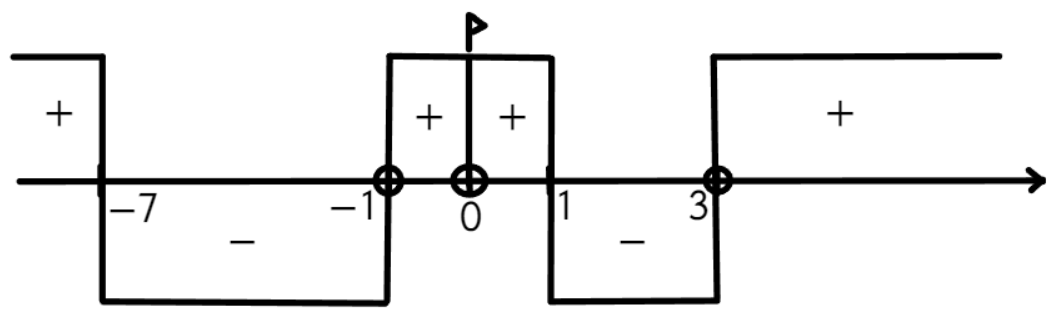
\includegraphics[scale=0.35]{ner9-63.png}}
\end{figure}\newpage\noindent
